\chapter{Precision Systems}
	This chapter is focused on system-related aspects that are relevant to \de{precision systems}, in particular related to the abbe, sine and cosine errors, the kinematic design and the flexure hinges.
	
\section{Alignment: Abbe, sine and cosine errors}
	
	Alignment errors are arising every time we need to align a measurement system and the subject of study: we have to be aware of this kind of error in order to detect them and control/reduce them. In particular the \de{Abbe} error arise every time there's an offset between the object to be measured and the system that perform the measure.
	
	Doing a low-volume production (or with high added value products) it's possible to rely on a manual inspection held by highly trained technician in order to ensure a certain level of quality; considering instead a mass production a handmade check of each component it's not possible due to a fully automated manufacturing and assembly for which there is a little space for adjustment: repeatability and precision must be designed into the product in order to have a high quality.
	
	\paragraph{Abbe's error} Common alignment errors are related to the \textbf{Abbe's error} associated  to it's principle stating that \textit{"the measurement line shall be collinear with the line of motion"}.
	
	\begin{SCfigure}[1][bht]
		\centering
		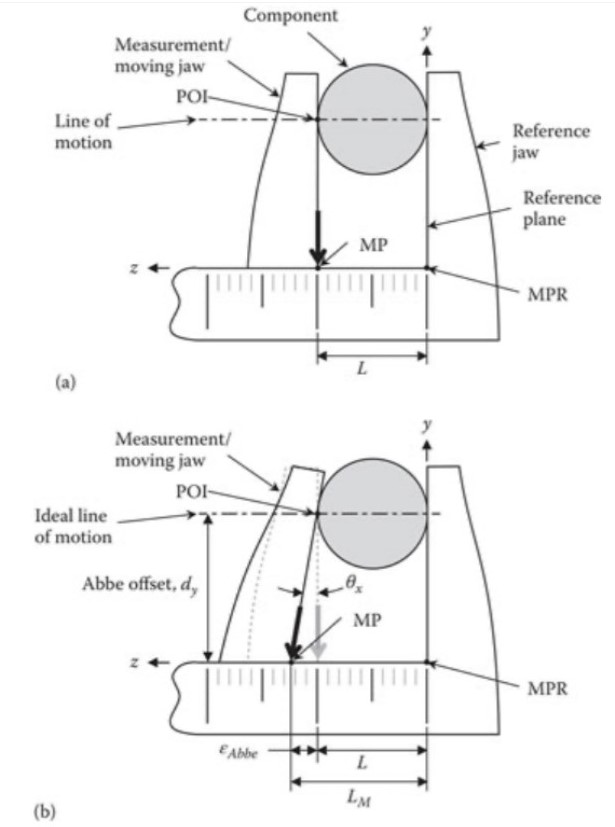
\includegraphics[width=6cm]{abbe-scheme}
		\caption{scheme used to understand the Abbe's error on a calliper. $(a)$ is a correct calliper while $(b)$ is affected by the error.} \label{fig:ps:abbescheme}
	\end{SCfigure}
	An example of this error can be seen in the calliper as in figure \ref{fig:ps:abbescheme}, where the goal is to measure the \textbf{Point of Interest} POI by reading the \textbf{Measurement Point} MP in respect to the Measurement Point \textbf{Reference} MPR. \\
	At a nominal level the two jaws of the calliper should be parallel, and so the point of interest is measured by only looking at the measurement point, but in reality misalignment are always present: this introduce an error $\abbe$ of the measurement point respect to the point of interest. Related to this error we can compute a linear relation but also an expression considering a second order term (that for low error alignment value $\theta_x$ can be neglected), obtaining
	\begin{equation}
		\abbe = d_y \tan\theta_x - \underbrace{L \left(\frac 1 {\cos\theta_x} - 1\right)}_\textrm{2nd ord. term}
	\end{equation}
	
	In reality things are even more complicated: Abbe's error are related to two angle in the 3D space, the so called \textbf{pith} and \textbf{yaw}
	\begin{equation}
	\begin{split}		
		\abbe & = d_y \tan\theta_x - L \left(\frac 1 {\cos\theta_x} - 1\right) + d_x \tan\theta_y - L \left(\frac 1 {\cos\theta_y} - 1\right) \\
		& = d_y \tan\theta_x + d_x\tan\theta_y - L\left( \frac 1 {\cos\theta_x} + \frac 1 {\cos\theta_y} - 2 \right)
	\end{split}
	\end{equation}
	
	\begin{SCfigure}[2][bht]
		\centering
		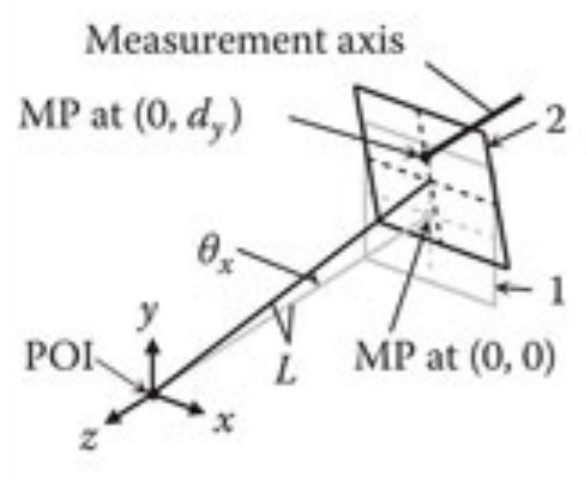
\includegraphics[width=3.5cm]{abbe-error}
		\caption{scheme used to understand the equation of the Abbe's error.} 
	\end{SCfigure}

	In order to eliminate the Abbe's error we can compensate by adding two more sensor (to determine $\theta_x,\theta_y$) that can determine the error $\abbe$. The same goal can be performed by analysing a sample problem: known it's value $L_m$, the computed measures is
	\[ L = L_m - d_y\tan\theta_x - d_x\tan\theta_y \]
	By evaluating this expression in two points (considering that an error, like $d_x\tan\theta_y$, can be consider negligible in respect to the other) by measuring an object more internal and external, we have a mathematical system that can be used in order to determine the unknown value $\theta_x$ and $L$. This method, in order to be successful, must consider that the angles $\theta_x$ and the length $L$ of the measure are invariant while changing the position of the sample.
	
	A smarter way to avoid the Abbe's error is just by doing a design choice minimizing the offset, so by making the line of motion collinear with the line of measurement.
	
	\paragraph{Cosine and sine error} The \de{cosine} error happens every time the measurement line is not parallel to the line of action. Considering the example of the measure of a length with a rule (as in figure \ref{fig:ps:cosineerror}) we can see that the measured length $L_m$ is different from the \textit{real} length $L$ of the object that we want to study, and in particular we can then evaluate the difference in order to define the cosine error $\varepsilon_{\cos}$:
	\begin{equation}
		L = L_m \cos\alpha \qquad \Rightarrow \quad \varepsilon_{\cos} = L_m - L = L_m \big(1-\cos\alpha\big)
	\end{equation}
	
	\begin{SCfigure}[1.3][bht]
		\centering
		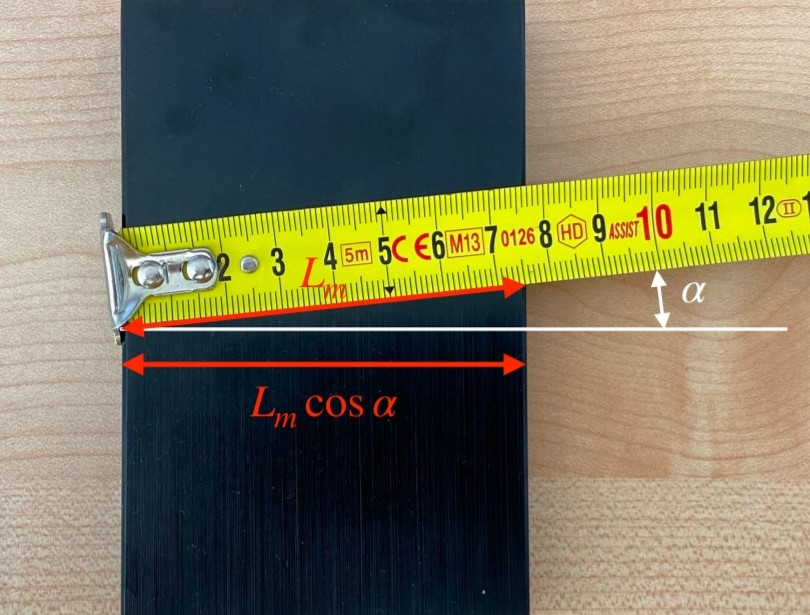
\includegraphics[width=5cm]{cosine-error}
		\caption{cosine error on a length measure.}  \label{fig:ps:cosineerror}
	\end{SCfigure}
	Extending the cosine error to a spatial environment we can compute  the error considering two angle $\alpha_x$ and $\alpha_y$ that can lead to an error:
	\begin{equation}
		\varepsilon_{\cos} = L_m\big(1-\cos\alpha_x\cos\alpha_y\big)
	\end{equation}
	\vspace{3mm}
	
	The \de{sine} error typically occurs when a physical contact is necessary for the measurement, like while dealing with the jaws of the calliper. By referring to figure \ref{fig:ps:sineerror} we can see that the error $\varepsilon_{\sin}$ is different in base of the geometry of the contact; considering as an example a flat-on-flat contact we can evaluate the error as
	\begin{equation}
		\varepsilon_{\sin} = \frac {w_z}2\sin\alpha_x + \frac{w_x}{2}\sin \alpha_z
	\end{equation}
	while considering instead a point contact the error reduces to the expression
	\begin{equation}
		\varepsilon_{\sin} = \frac {w_z}2\big(1-\cos\alpha_x\big) + \frac{w_x}{2}\big(1-\cos\alpha_z\big) = \frac{w_z}{2}\big(2-\cos\alpha_x-\cos\alpha_z\big)
	\end{equation}	
	
	
	\begin{SCfigure}[1.3][bht]
		\centering
		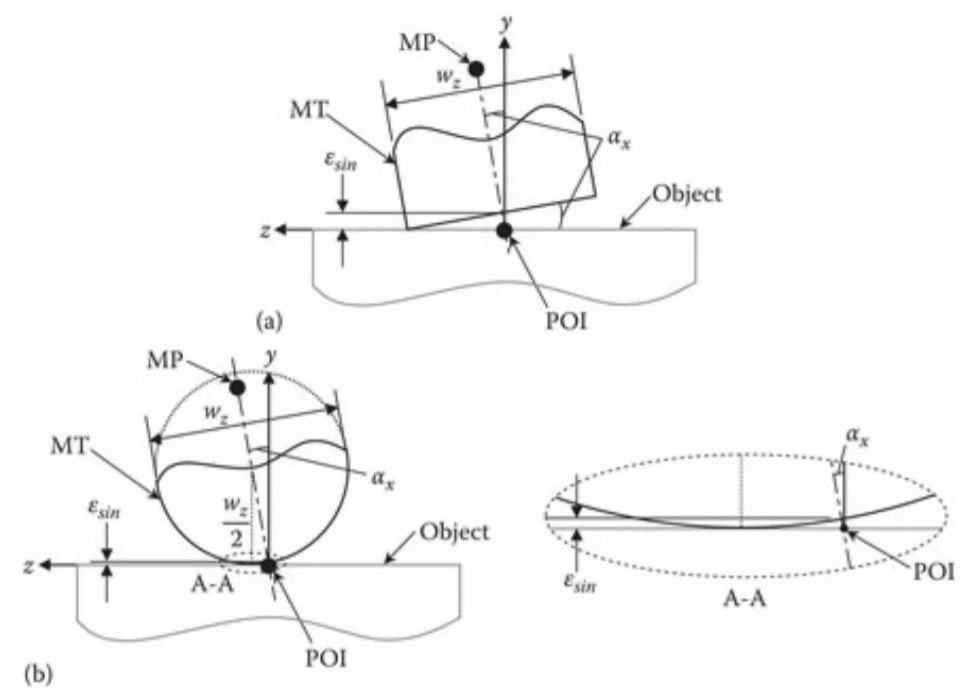
\includegraphics[width=5cm]{sine-error}
		\caption{sine error on a surface measure considering a flat-on-flat contact $(a)$ or a point contact $(b)$.}  \label{fig:ps:sineerror}
	\end{SCfigure}

	\paragraph{Alignment errors} In general Abbe's, cosine and sine errors are not mutually exclusive, so they can occur at the same time (Abbe's related to the offset, cosine due to a scale line not parallel to the  line of motion and the sine related to the angle between the moving jaw and the object).
	
	While designing measurement system it's important to determine all the specification that are useful to calculate the error factors that should be less then a decided value; this gives a suggestion on how to chose tolerances of the products.
	
	\begin{figure}[bht]
		\centering
		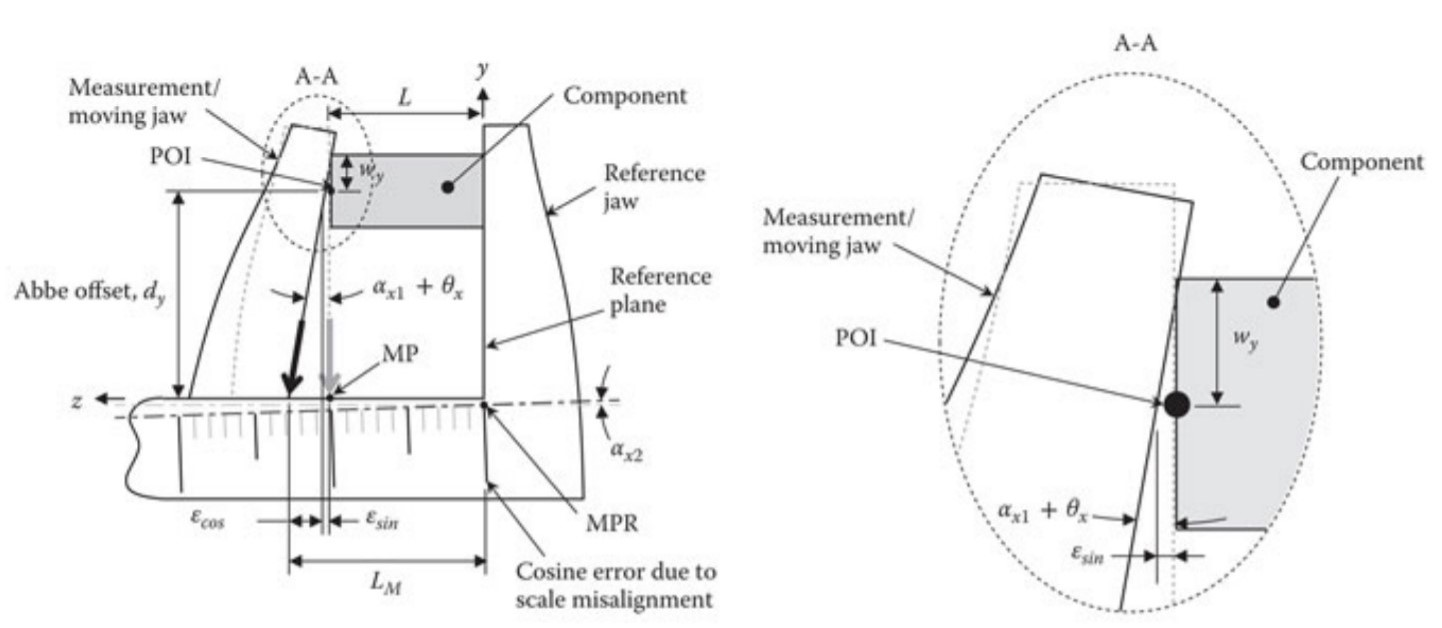
\includegraphics[width=10cm]{comb-errors}
		\caption{example of the combination of Abbe's, cosine and sine errors in a calliper.}
	\end{figure}
	
\section{Kinematics}
	
	In order to have a repeatable positioning it's important to minimize the internal stress by pursuing an isostatic design. When designing a system the kinematic analysis provides an understanding between the functional relationship between parts of mechanism, on how these parts are interconnected and how they move relative to each other.
	
	For example an unilateral constraint is represented by an inequality such $f(x,y,z) \geq 0$: in this step we usually consider bodies as \textbf{rigid}, so by considering part that are stiff enough in order to consider their deformation negligible in respect to the typical range of motion of the system. In precise machine it's important to consider all contact as rigid. \\
	In kinematic design we can assume that each	point of contact between two rigid bodies corresponds to a mutual constraint. In general if $f_j$ is the number of degrees of freedom of a joint $j$ having $n_{p_j}$ lowest number of contact point, than it's true that
	\begin{equation}
	\begin{split}
		\textrm{planar kinematics:}& \qquad f_j = 3 - n_{p_j} \\
		\textrm{spatial kinematics:}& \qquad f_j = 6 - n_{p_j} \\
	\end{split}
	\end{equation}
	
	Considering the more complex scenario of two line (straight or arcuate) contact, this is kinematically equivalent to two point constraints applied to any two different points along the contact line. 
	
	\begin{SCfigure}[2][bht]
		\centering
		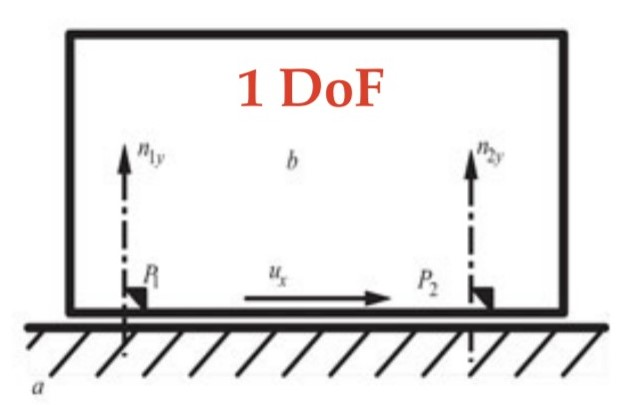
\includegraphics[width=3.5cm]{planar-contact}
		\caption{the contact of a body with straight line on a straight surface leads to two point constrains in order to have 1 degrees of freedom.}
	\end{SCfigure}
	
	\paragraph{Mobility of mechanisms} Considering now  a combination of $n$ rigid bodies constrained by $j$ joints can lead to a movable or immovable system. The net mobility of the mechanism is its number of degrees of freedom and can be calculated according to Tchebytchev as
	\begin{equation}
		M = D\big(n-1-j\big) +\sum_i f_i = D\big(n-1\big) -\sum_j n_{p_j}
	\end{equation}
	where $D= 6$ for spatial mechanisms while $D= 3$ for planar kinematics. If $M>0$ then the mechanism is movable, for $M = 0$ the system is immovable while $M < 0$ it's over-constrained and so, in a real application, the structure will be subjected to unknown internal stresses that cannot be quantified (and so leading to imprecision).
	
	The Tchebytchev should be used with caution when dealing with systems that present singularities that can be determined by considering the position of the instantaneous centers of rotation of the bodies composing the system. Given a body $a$, it's instantaneous center of rotation in respect to the body $b$ is written as $P_{ab}$ and depends on the local configuration of the system. Every time that the center $P_{ij}$ goes to infinity, than the related configuration is singular and the Tchebytchev mobility calculation isn't correct.
	
	\paragraph{Over and under-constrained mechanisms} Under od over-constrained mechanisms can have unexpected side-effects that are often resulting in a lack of repeatability (unknown deformation of the system or unknown motion of some elements). As a consequence in precision engineering it is relevant to rely on kinematic design (which means exact constraint design) in order to have an isostatic system.
	
	\begin{figure}[bht]
		\centering
		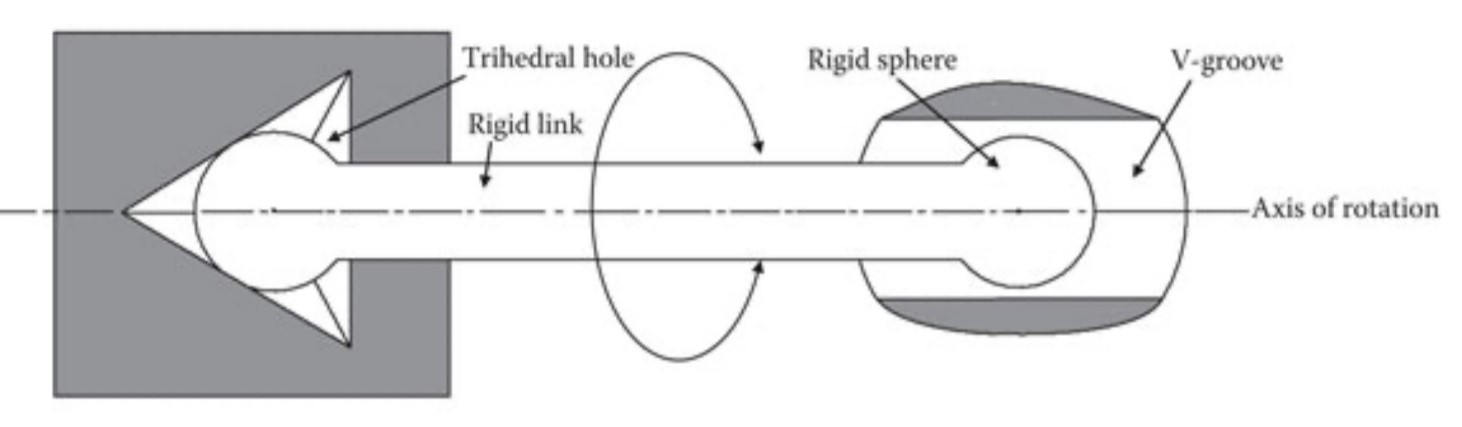
\includegraphics[width=7cm]{contactpointexample}
		\caption{example of a kinematic design of a rotary shaft.}
		\label{fig:ps:contactpointexample}
	\end{figure}

	Considering the example in figure \ref{fig:ps:contactpointexample} we can see that the tetrahedral groove determines 3 contact point, while the V groove add other 2, by determining a 1 degree of freedom of the shaft that's so free to rotate on it's axes. By replacing the V groove with another tetrahedral we have a $M=0$ and in order to have a mechanism that rotate we have to ensure that the shaft length is equal to the hole distance. An implementation of the previous kinematic design can be made with swivel ball (related to the V groove) and roller (tetrahedral) bearing as in figure \ref{fig:ps:contactsolution}.
	
	\begin{SCfigure}[2][bht]
		\centering
		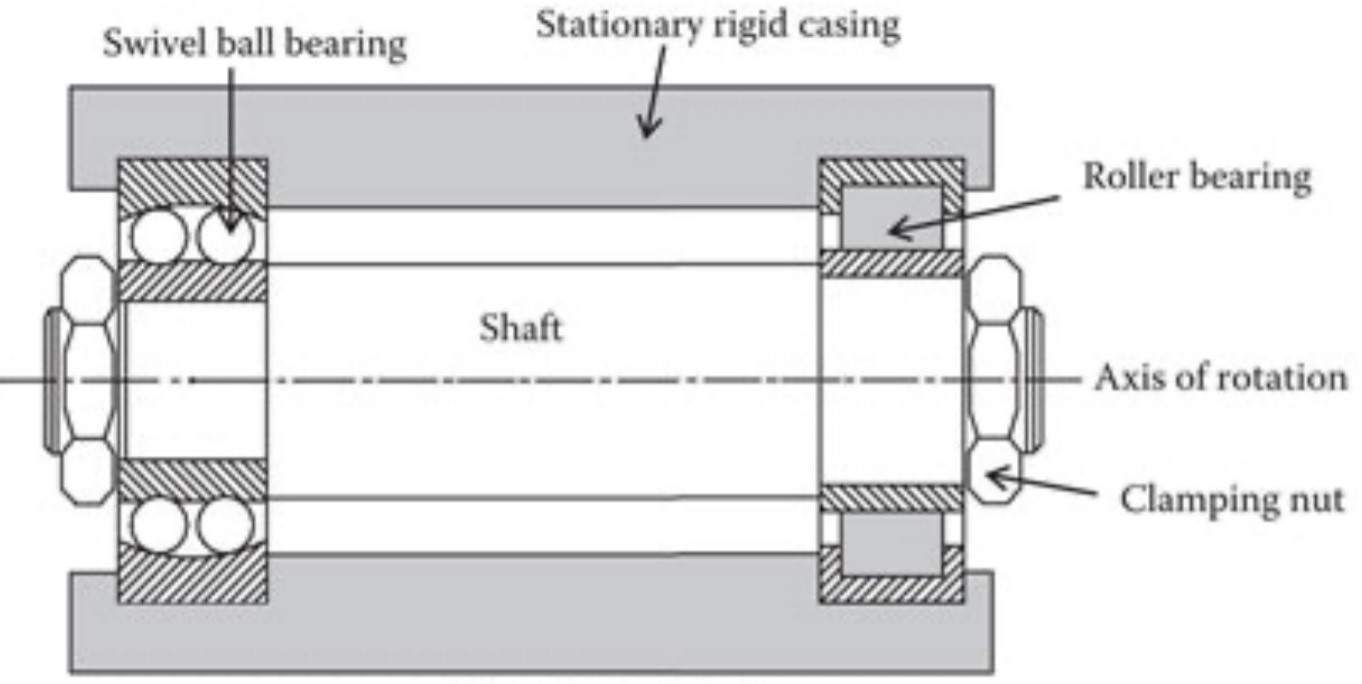
\includegraphics[width=6cm]{contactpointexample-sol}
		\caption{practical solution of the kinematic design of a rotary shaft drawn in figure \ref{fig:ps:contactpointexample}.}
		\label{fig:ps:contactsolution}
	\end{SCfigure}
	
	In general any deviation from purely kinematic design requires tighter tolerances and more stable materials that leads to increasing costs. In purely kinematic design it's required to use the minimum number of contact points that, as trade-off, increases the internal stress (and so decreasing the load capacity).
	
	\paragraph{Pseudo-kinematic design} To increase the load capacity we can use the so called \de{pseudo-kinematic design} by increasing the contact area while still providing constrains that are similar that are kinematic equivalent.
	
	\paragraph{Elastic averaging} Another approach that can be used to reduce the effects of machining inaccuracy is to use a large number of compliant coupling in order to spread the errors on a large area.	An example of this technique can be seen in figure \ref{fig:ps:elasticaveraging}.
	
	\begin{figure}[bht]
		\centering
		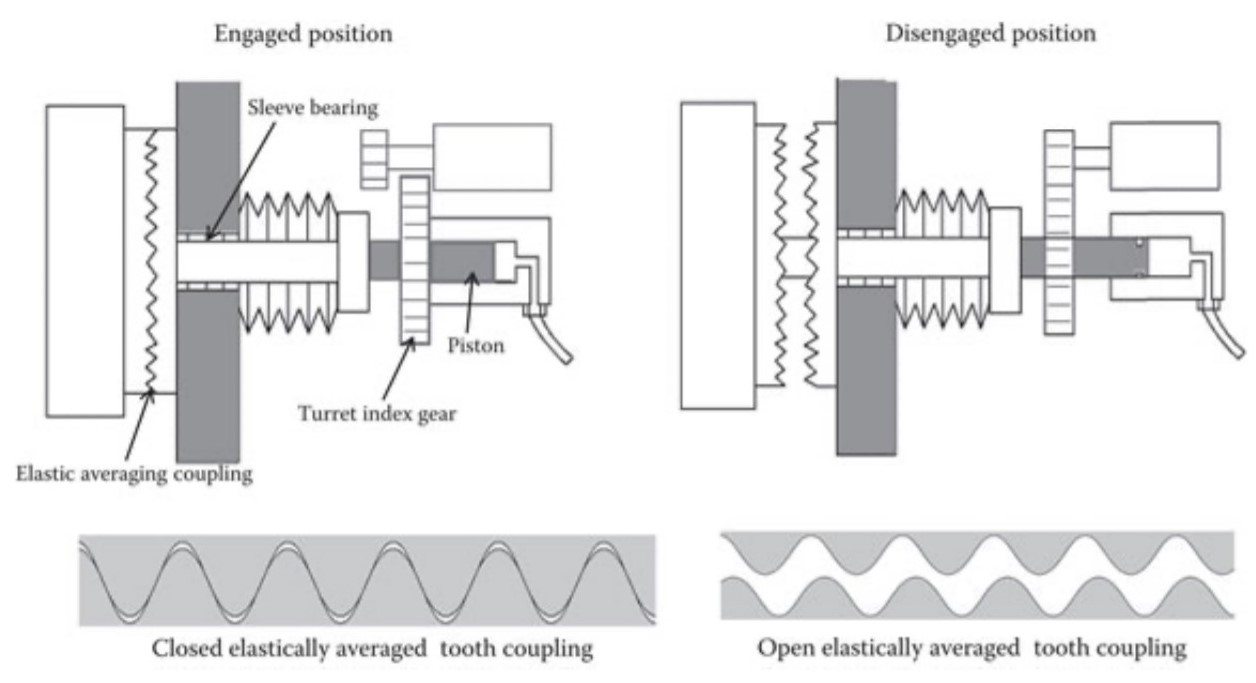
\includegraphics[width=9cm]{elasticavereging}
		\caption{example of a system that uses elastic averaging in order to better create a kinematic connection between two components.}
		\label{fig:ps:elasticaveraging}
	\end{figure}
	
	\subsection{Kinematic couplings}
		When designing a precision assembly we often need to precisely locate two subsystems respect to each other; sometimes we also want to isolate effects of strains acting on the frame element from a carried subsystem. In all this cases the coupling must be kinematic (by so determining a mobility $M=0$) in order to decouple the carried subsystem from effects of the carrier (like mechanical and thermals strains, manufacturing errors...).
		
		One of the most common type of kinematic coupling is the \textbf{Kelvin clamp} as in figure \ref{fig:ps:kelvinclamp}. In general good coupling design shall avoid overconstrained geometries (as example a pillar that have to support a high load, we don't use a pure flat surface but only a perimeter part of the cross section in order to minimize the surface in contact).
		
		\begin{SCfigure}[2][bht]
			\centering
			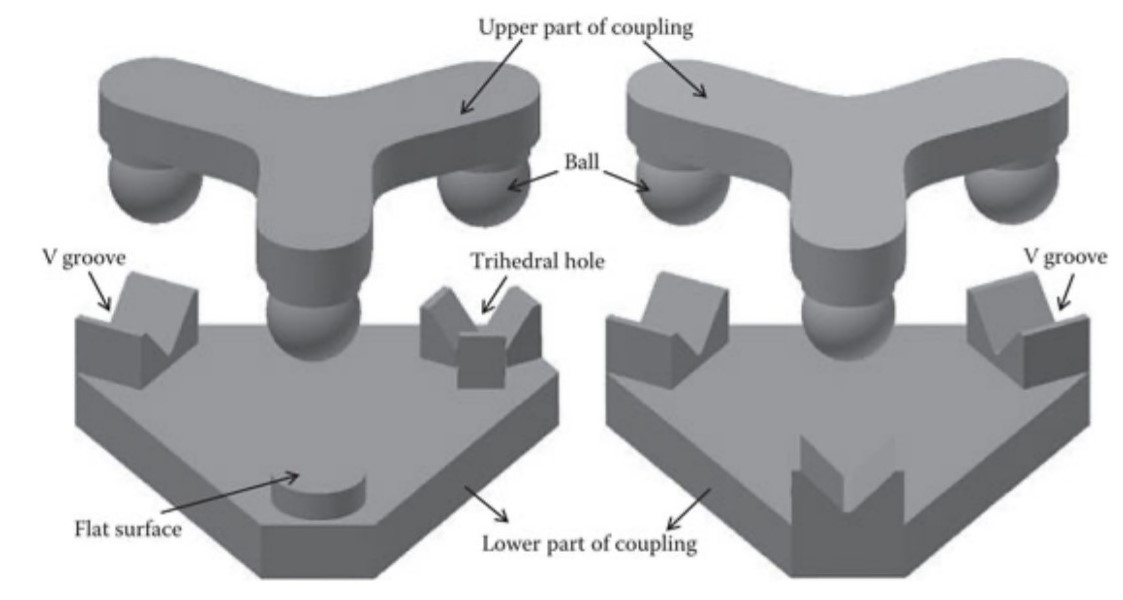
\includegraphics[width=6.5cm]{kelvinclamp}
			\caption{Kelvin clamp of type I (on the left) and type II (right).} 
			\label{fig:ps:kelvinclamp}
		\end{SCfigure}
		
		\paragraph{Hertzian contacts} In order to describe the elastic interaction between contact point we can use the theory of the \de{Hertzian contacts} that allows to compute the pressure $p(r)$ and contact stiffness $K_n$ of a sphere on a sphere (or on a plane considering $R_2$ that tends to infinity). In particular the pressure on the surface and the contact stiffness can be calculated, depending on the applied force $F_n$, as
		\begin{equation}
			p(r) = p_0 \sqrt{1- \frac{r^2}{a^2}} \qquad K_n = \frac{dF_n}{d\delta} = 2\overline E \sqrt{\delta R}
		\end{equation}
		when the parameters can be computed as
		\[ p_0 = \sqrt[3]{\frac{6 F_n E^2}{\pi^3 R^2}} \qquad a = \sqrt[3]{\frac{3F_n R}{4\overline E}} \qquad \delta = \frac{a^2}{R} = \sqrt[3]{ \frac{9F_n^2}{16\overline E^2 R} } \]
		In order to compute the average $\overline E$ of the Young modules the following expression must be considered:
		\[\frac 1 {\overline E} = \frac{1-\nu_1^2}{E_1} + \frac{1-\nu_2^2}{E_2} \]
		\textbf{FIGURA DEL CONTATTO, SLIDE 41}
		
		Considering instead the contact of a cylinder on a cylinder the surface pressure depended from the deviation $x$ on the ideal contact line and is equal to
		\begin{equation}
			p(x) = p_0 \sqrt{1- \frac{r^2}{b^2}}
		\end{equation}
		where
		\[ p_0 = \frac{2F_n}{\pi b L } = \sqrt{\frac{F_b\overline E}{\pi RL}} \qquad b = \sqrt{\frac{4F_nR}{\pi \overline E L}} \qquad \delta = \frac{F_n}{\pi \overline E L} \left[ 1 + \ln \left(\frac{\pi L^3\overline E}{PR}\right) \right] \]
	
	
		\paragraph{Dowel pins} A common need is to precisely mount a plate onto a base and this operation is often performed by the \textbf{dowel pins}: each pin locks one degree of freedom on the plane, so 3 pins can be used to kinematic constrain a plate in a planar kinematic. In reality this pins are unilateral constrains and so a 4-th locking point is needed.
		
		\textbf{DISCORSO SUL CALCOLO DEI MOMENTI ROTAZIONE PER CAPIRE SE I PIN SONO SUFFICIENTI, MAGARI RIVEDERE LEZIONE}
	

\section{Flexure hinges}
	\de{Flexure hinges} are made as a substitute to the conventional rotational joint by using an elastic deformation of a single element (so with no movable part) that allows to have a more repeatable motion of the mechanism.
	
	
	
	
	
	
	
	
	
	
	
	
	
	
	
	
	
	
	
	
	
	
	
	
	
	
	
	
	
	
	
	
	
	
	
	
	
	
	
	
	
	
	